

% \tikzset{every picture/.style={line width=0.75pt}} %set default line width to 0.75pt

% \begin{tikzpicture}[x=0.75pt,y=0.75pt,yscale=-1,xscale=1]
% %uncomment if require: \path (0,300); %set diagram left start at 0, and has height of 300

% %Shape: Circle [id:dp9841098010993801]
% \draw   (40,140) .. controls (40,128.95) and (48.95,120) .. (60,120) .. controls (71.05,120) and (80,128.95) .. (80,140) .. controls (80,151.05) and (71.05,160) .. (60,160) .. controls (48.95,160) and (40,151.05) .. (40,140) -- cycle ;
% %Straight Lines [id:da80001405628028]
% \draw    (80,140) -- (118,140) ;
% \draw [shift={(120,140)}, rotate = 180] [color={rgb, 255:red, 0; green, 0; blue, 0 }  ][line width=0.75]    (6.56,-1.97) .. controls (4.17,-0.84) and (1.99,-0.18) .. (0,0) .. controls (1.99,0.18) and (4.17,0.84) .. (6.56,1.97)   ;
% %Shape: Circle [id:dp7651396635784946]
% \draw   (120,140) .. controls (120,128.95) and (128.95,120) .. (140,120) .. controls (151.05,120) and (160,128.95) .. (160,140) .. controls (160,151.05) and (151.05,160) .. (140,160) .. controls (128.95,160) and (120,151.05) .. (120,140) -- cycle ;
% %Rounded Rect [id:dp8846805761851559]
% \draw   (30,117.89) .. controls (30,113.53) and (33.53,110) .. (37.89,110) -- (162.11,110) .. controls (166.47,110) and (170,113.53) .. (170,117.89) -- (170,162.11) .. controls (170,166.47) and (166.47,170) .. (162.11,170) -- (37.89,170) .. controls (33.53,170) and (30,166.47) .. (30,162.11) -- cycle ;
% %Shape: Circle [id:dp8490824743149163]
% \draw   (120,60) .. controls (120,48.95) and (128.95,40) .. (140,40) .. controls (151.05,40) and (160,48.95) .. (160,60) .. controls (160,71.05) and (151.05,80) .. (140,80) .. controls (128.95,80) and (120,71.05) .. (120,60) -- cycle ;
% %Straight Lines [id:da3858630888275081]
% \draw    (210,140) -- (210,122) ;
% \draw [shift={(210,120)}, rotate = 450] [color={rgb, 255:red, 0; green, 0; blue, 0 }  ][line width=0.75]    (6.56,-1.97) .. controls (4.17,-0.84) and (1.99,-0.18) .. (0,0) .. controls (1.99,0.18) and (4.17,0.84) .. (6.56,1.97)   ;
% %Straight Lines [id:da26074500801995315]
% \draw    (210,60) -- (210,78) ;
% \draw [shift={(210,80)}, rotate = 270] [color={rgb, 255:red, 0; green, 0; blue, 0 }  ][line width=0.75]    (6.56,-1.97) .. controls (4.17,-0.84) and (1.99,-0.18) .. (0,0) .. controls (1.99,0.18) and (4.17,0.84) .. (6.56,1.97)   ;
% %Straight Lines [id:da6758238298583736]
% \draw    (160,60) -- (210,60) ;
% %Shape: Circle [id:dp6353953977655111]
% \draw   (190,100) .. controls (190,88.95) and (198.95,80) .. (210,80) .. controls (221.05,80) and (230,88.95) .. (230,100) .. controls (230,111.05) and (221.05,120) .. (210,120) .. controls (198.95,120) and (190,111.05) .. (190,100) -- cycle ;
% %Straight Lines [id:da9061844154631766]
% \draw    (160,140) -- (210,140) ;
% %Straight Lines [id:da187317559248537]
% \draw  [dash pattern={on 0.84pt off 2.51pt}]  (230,100) -- (268,100) ;
% \draw [shift={(270,100)}, rotate = 180] [color={rgb, 255:red, 0; green, 0; blue, 0 }  ][line width=0.75]    (6.56,-1.97) .. controls (4.17,-0.84) and (1.99,-0.18) .. (0,0) .. controls (1.99,0.18) and (4.17,0.84) .. (6.56,1.97)   ;
% %Shape: Circle [id:dp0952580832819716]
% \draw   (270,100) .. controls (270,88.95) and (278.95,80) .. (290,80) .. controls (301.05,80) and (310,88.95) .. (310,100) .. controls (310,111.05) and (301.05,120) .. (290,120) .. controls (278.95,120) and (270,111.05) .. (270,100) -- cycle ;
% %Straight Lines [id:da6354202649322243]
% \draw  [dash pattern={on 0.84pt off 2.51pt}]  (170,150) -- (290,150) ;
% %Straight Lines [id:da051339880414786876]
% \draw  [dash pattern={on 0.84pt off 2.51pt}]  (290,150) -- (290,122) ;
% \draw [shift={(290,120)}, rotate = 450] [color={rgb, 255:red, 0; green, 0; blue, 0 }  ][line width=0.75]    (6.56,-1.97) .. controls (4.17,-0.84) and (1.99,-0.18) .. (0,0) .. controls (1.99,0.18) and (4.17,0.84) .. (6.56,1.97)   ;

% % Text Node
% \draw (54,135) node [anchor=north west][inner sep=0.75pt]    {$\boldsymbol{z}$};
% % Text Node
% \draw (133,133) node [anchor=north west][inner sep=0.75pt]    {$\boldsymbol{\tilde{x}}$};
% % Text Node
% \draw (133,55) node [anchor=north west][inner sep=0.75pt]    {$\boldsymbol{x}$};
% % Text Node
% \draw (202,93) node [anchor=north west][inner sep=0.75pt]    {$D$};
% % Text Node
% \draw (283,92) node [anchor=north west][inner sep=0.75pt]    {$\mathcal{L}$};
% % Text Node
% \draw (91,147.4) node [anchor=north west][inner sep=0.75pt]    {$G$};


% \end{tikzpicture}




\tikzset{every picture/.style={line width=0.75pt}} %set default line width to 0.75pt

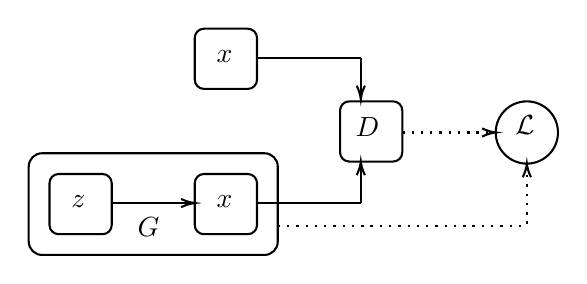
\begin{tikzpicture}[x=0.75pt,y=0.75pt,yscale=-1,xscale=1]
%uncomment if require: \path (0,300); %set diagram left start at 0, and has height of 300

%Straight Lines [id:da28863933254527985]
\draw [line width=0.75]    (80,119) -- (118,119) ;
\draw [shift={(120,119)}, rotate = 180] [color={rgb, 255:red, 0; green, 0; blue, 0 }  ][line width=0.75]    (6.56,-1.97) .. controls (4.17,-0.84) and (1.99,-0.18) .. (0,0) .. controls (1.99,0.18) and (4.17,0.84) .. (6.56,1.97)   ;
%Rounded Rect [id:dp309037838449697]
\draw  [line width=0.75]  (40,101.44) .. controls (40,97.88) and (42.88,95) .. (46.44,95) -- (153.56,95) .. controls (157.12,95) and (160,97.88) .. (160,101.44) -- (160,137.56) .. controls (160,141.12) and (157.12,144) .. (153.56,144) -- (46.44,144) .. controls (42.88,144) and (40,141.12) .. (40,137.56) -- cycle ;
%Straight Lines [id:da5648922428474259]
\draw [color={rgb, 255:red, 0; green, 0; blue, 0 }  ,draw opacity=1 ][line width=0.75]    (200,119) -- (200,101) ;
\draw [shift={(200,99)}, rotate = 450] [color={rgb, 255:red, 0; green, 0; blue, 0 }  ,draw opacity=1 ][line width=0.75]    (6.56,-1.97) .. controls (4.17,-0.84) and (1.99,-0.18) .. (0,0) .. controls (1.99,0.18) and (4.17,0.84) .. (6.56,1.97)   ;
%Straight Lines [id:da05240629004366304]
\draw [line width=0.75]    (200,49) -- (200,67) ;
\draw [shift={(200,69)}, rotate = 270] [color={rgb, 255:red, 0; green, 0; blue, 0 }  ][line width=0.75]    (6.56,-1.97) .. controls (4.17,-0.84) and (1.99,-0.18) .. (0,0) .. controls (1.99,0.18) and (4.17,0.84) .. (6.56,1.97)   ;
%Straight Lines [id:da8495437226033926]
\draw [line width=0.75]    (150,49) -- (200,49) ;
%Straight Lines [id:da7495630290122488]
\draw [color={rgb, 255:red, 0; green, 0; blue, 0 }  ,draw opacity=1 ][line width=0.75]    (150,119) -- (200,119) ;
%Straight Lines [id:da026211187325514862]
\draw [line width=0.75]  [dash pattern={on 0.84pt off 2.51pt}]  (220,85) -- (263,85) ;
\draw [shift={(265,85)}, rotate = 180] [color={rgb, 255:red, 0; green, 0; blue, 0 }  ][line width=0.75]    (6.56,-1.97) .. controls (4.17,-0.84) and (1.99,-0.18) .. (0,0) .. controls (1.99,0.18) and (4.17,0.84) .. (6.56,1.97)   ;
%Shape: Circle [id:dp2250548008814215]
\draw   (265,85) .. controls (265,76.72) and (271.72,70) .. (280,70) .. controls (288.28,70) and (295,76.72) .. (295,85) .. controls (295,93.28) and (288.28,100) .. (280,100) .. controls (271.72,100) and (265,93.28) .. (265,85) -- cycle ;
%Straight Lines [id:da35112695712380004]
\draw [line width=0.75]  [dash pattern={on 0.84pt off 2.51pt}]  (160,130) -- (280,130) ;
%Straight Lines [id:da8869405404857167]
\draw [line width=0.75]  [dash pattern={on 0.84pt off 2.51pt}]  (280,129) -- (280,102) ;
\draw [shift={(280,100)}, rotate = 450] [color={rgb, 255:red, 0; green, 0; blue, 0 }  ][line width=0.75]    (6.56,-1.97) .. controls (4.17,-0.84) and (1.99,-0.18) .. (0,0) .. controls (1.99,0.18) and (4.17,0.84) .. (6.56,1.97)   ;
%Rounded Rect [id:dp993659051393138]
\draw  [color={rgb, 255:red, 0; green, 0; blue, 0 }  ,draw opacity=1 ][line width=0.75]  (50,109.44) .. controls (50,106.99) and (51.99,105) .. (54.44,105) -- (75.56,105) .. controls (78.01,105) and (80,106.99) .. (80,109.44) -- (80,129.56) .. controls (80,132.01) and (78.01,134) .. (75.56,134) -- (54.44,134) .. controls (51.99,134) and (50,132.01) .. (50,129.56) -- cycle ;
%Rounded Rect [id:dp010339036488199005]
\draw  [color={rgb, 255:red, 0; green, 0; blue, 0 }  ,draw opacity=1 ][line width=0.75]  (120,109.44) .. controls (120,106.99) and (121.99,105) .. (124.44,105) -- (145.56,105) .. controls (148.01,105) and (150,106.99) .. (150,109.44) -- (150,129.56) .. controls (150,132.01) and (148.01,134) .. (145.56,134) -- (124.44,134) .. controls (121.99,134) and (120,132.01) .. (120,129.56) -- cycle ;
%Rounded Rect [id:dp8207653979046976]
\draw  [line width=0.75]  (120,39.44) .. controls (120,36.99) and (121.99,35) .. (124.44,35) -- (145.56,35) .. controls (148.01,35) and (150,36.99) .. (150,39.44) -- (150,59.56) .. controls (150,62.01) and (148.01,64) .. (145.56,64) -- (124.44,64) .. controls (121.99,64) and (120,62.01) .. (120,59.56) -- cycle ;
%Rounded Rect [id:dp7258941426050629]
\draw  [color={rgb, 255:red, 0; green, 0; blue, 0 }  ,draw opacity=1 ][line width=0.75]  (190,74.44) .. controls (190,71.99) and (191.99,70) .. (194.44,70) -- (215.56,70) .. controls (218.01,70) and (220,71.99) .. (220,74.44) -- (220,94.56) .. controls (220,97.01) and (218.01,99) .. (215.56,99) -- (194.44,99) .. controls (191.99,99) and (190,97.01) .. (190,94.56) -- cycle ;

% Text Node
\draw (59,114) node [anchor=north west][inner sep=0.75pt]    {$\boldsymbol{z}$};
% Text Node
\draw (129,114) node [anchor=north west][inner sep=0.75pt]    {$\boldsymbol{x}$};
% Text Node
\draw (129,44) node [anchor=north west][inner sep=0.75pt]    {$\boldsymbol{x}$};
% Text Node
\draw (196,76.4) node [anchor=north west][inner sep=0.75pt]    {$D$};
% Text Node
\draw (273,75.4) node [anchor=north west][inner sep=0.75pt]    {$\mathcal{L}$};
% Text Node
\draw (91,124.4) node [anchor=north west][inner sep=0.75pt]    {$G$};


\end{tikzpicture}